\chapter{Risultati}
\label{cap:3}
I risultati finali sono suddivisi nelle due caratteristiche su cui è stata sviluppata l'analisi dei dati.
Sono quindi presenti una sezione relativa ai tempi di esecuzione e una sulla memoria fisica sfruttata. 
La descrizione delle relazioni più interessanti è, inoltre, accompagnata dall'utilizzo di alcuni tra i grafici elaborati durante lo studio statistico.

In sede di analisi sono stati usati subset con dimensione minima di centomila.

\section{Tempi di esecuzione}
L'indagine sui tempi di esecuzione, come spiegato nel paragrafo \ref{sbsec:Te}, è stata condotta approfondendo le seguenti relazioni: i tempi di esecuzione per le regole, la durata complessiva del processo e i tempi impiegati per intervalli differenti con lo stesso numero di sequenze. 
Questa sezione si occuperà di presentare gli esiti finali più rilevanti di ognuno di tali aspetti.

\subsection{Tempi e regole}
Le regole previste dal procedimento hanno concentrato l'analisi su due campi, uno relativo a quei processi che non dipendono dal tipo di dati considerato e uno relativo a quelli che invece dipendono. 
Considerando le prime, si può notare dalla figura \ref{fig:Tind} come l'unico processo significativo sia l'indicizzazione dello human reference per BWA, mentre le rimanenti non influiscano in alcun modo. 
In più, la differenza tra le potenze computazionali è netta già da questa figura, dato che tra il nodo migliore e il peggiore vi è uno scarto di più di un'ora.
\begin{figure}[H]
\centering
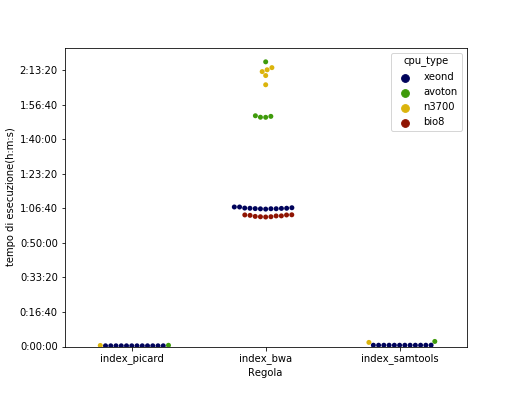
\includegraphics[scale=0.46]{Tind.png}
\caption{Tempi di esecuzione per le regole indipendenti dal subset.}
\label{fig:Tind}
\end{figure}
Nonostante la durata per l'indicizzazione sia notevole, questa fase è riprodotta una sola volta per tutte le successive simulazioni, visto che è riferita solamente al genoma umano di riferimento.

Passando alle regole dipendenti, i grafici riportati nelle figure \ref{subfig:BB}, \ref{subfig:Map}, \ref{subfig:MD}, \ref{subfig:Rlg} e \ref{subfig:SP} mostrano i vari andamenti per la grandezza dei subset.

Per ciascuna figura è anche riportata una tabella con i dettagli delle rigressioni lineari effetuate per descrivere il tempo di esecuzione in funzione del numero di sequenze lette.
La regressione è stata effettuata con il metodo di Theil-Sen.
Questo metodo implica una regressione lineare robusta, ovvero che non risente della presenza di \textit{outlier} nei dati.

Nelle tabelle è riportato l'intervallo di confidenza della pendenza della retta.
Visto che nessuno di questi intervalli di confidenza contiene lo zero, per tutte le regole vi è una dipendenza significativa fra il numero di sequenze ed il tempo impiegato.

\begin{figure}[H]
\centering
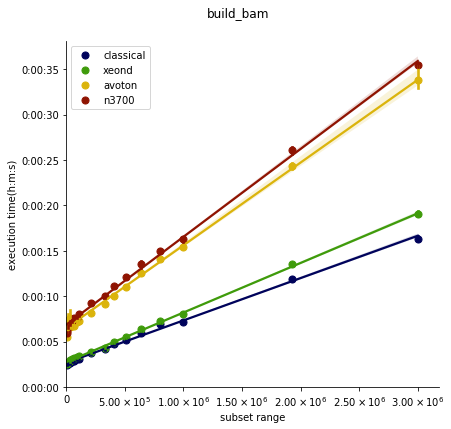
\includegraphics[scale=0.7]{build_bam.png}
\captionof{figure}{Tempi per Build BAM.}
\label{subfig:BB}
\end{figure}

\begin{table}[H]
    \centering
	\begin{tabular}{lrrrr}
	\toprule
	{} &         pendenza & intercetta &     min pendenza &     max pendenza \\
	\text{tipo di cpu} & $\frac{secondi}{\text{\num{e6} letture}}$ & $secondi$ & $\frac{secondi}{\text{\num{e6} letture}}$ & $\frac{secondi}{\text{\num{e6} letture}}$ \\
	\midrule
	avoton   & {9.2} &        6.4 &   {9} & {9.5} \\
	bio8     & {4.4} &        3.1 & {4.4} & {4.4} \\
	n3700    & {9.4} &        7.4 & {9.3} & {9.5} \\
	xeond    & {5.3} &          3 & {5.3} & {5.3} \\
	\bottomrule
	\end{tabular}
	\caption{Dettagli retta di fit per Build BAM.}
	\label{tab:Bb}
\end{table}

\begin{figure}[H]
\centering
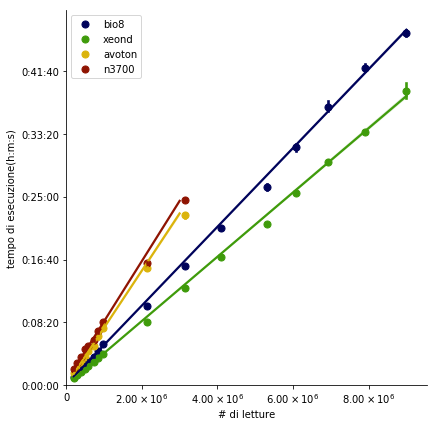
\includegraphics[scale=0.7]{mapping.png}	
\captionof{figure}{Tempi per Mapping.}
\label{subfig:Map}
\end{figure}

\begin{table}[H]
	\centering
	\begin{tabular}{lrrrr}
	\toprule
	{} &         pendenza & intercetta &     min pendenza &     max pendenza \\
	\text{tipo di cpu} & $\frac{secondi}{\text{\num{e6} letture}}$ & $secondi$ & $\frac{secondi}{\text{\num{e6} letture}}$ & $\frac{secondi}{\text{\num{e6} letture}}$ \\
	\midrule
	avoton   &{440} &        6.8 &{430} &{45} \\
	bio8     &{310} &        7.9 &{310} &{310} \\
	n3700    &{470} &         24 &{470} &{480} \\
	xeond    &{250} &       -3.3 &{250} &{250} \\
	\bottomrule
	\end{tabular}
    \caption{Dettagli retta di fit per Mapping.}
    \label{tab:Mp}
\end{table}

\begin{figure}[H]
\centering
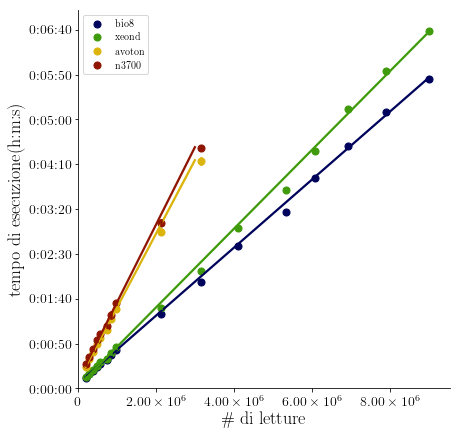
\includegraphics[scale=0.7]{mark_duplicates.png}
\captionof{figure}{Tempi per Mark Duplicates.}
\label{subfig:MD}
\end{figure}

\begin{table}[H]
    \centering    
	\begin{tabular}{lrrrr}
	\toprule
	{} &         pendenza & intercetta &     min pendenza &     max pendenza \\
	\text{tipo di cpu} & $\frac{secondi}{\text{\num{e6} letture}}$ & $secondi$ & $\frac{secondi}{\text{\num{e6} letture}}$ & $\frac{secondi}{\text{\num{e6} letture}}$ \\
	\midrule
	avoton   &{81} &        7.9 &{81} &{82} \\
	bio8     &{38} &        4.7 &{38} &{38} \\
	n3700    &{86} &        8.9 &{85} &{87} \\
	xeond    &{44} &        2.4 &{43} &{44} \\
	\bottomrule
	\end{tabular}
    \caption{Dettagli retta di fit per Mark Duplicates.}
	\label{tab:Md}
\end{table}

\begin{figure}[H]
\centering
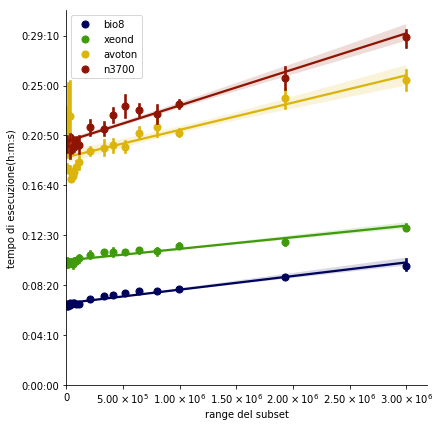
\includegraphics[scale=0.7]{realigner.png}
\captionof{figure}{Tempi per i tempi di Realigner.}
\label{subfig:Rlg}
\end{figure}

\begin{table}[H]
	\centering
	\begin{tabular}{lrrrr}
	\toprule
	{} &         pendenza & intercetta &     min pendenza &     max pendenza \\
	\text{tipo di cpu} & $\frac{secondi}{\text{\num{e6} letture}}$ & $secondi$ & $\frac{secondi}{\text{\num{e6} letture}}$ & $\frac{secondi}{\text{\num{e6} letture}}$ \\
	\midrule
	avoton   &{130} &    \num{1.2e+03} &{110} &{160} \\
	bio8     &{38} &    \num{4.5e+02} &{36} &{39} \\
	n3700    &{150} &    \num{1.3e+03} &{120} &{170} \\
	xeond    &{38} &    \num{6.8e+02} &{36} &  {40} \\
	\bottomrule
	\end{tabular}
    \caption{Dettagli retta di fit per Realigner.}
	\label{tab:Rlg}
\end{table}

\begin{figure}[H]
\centering
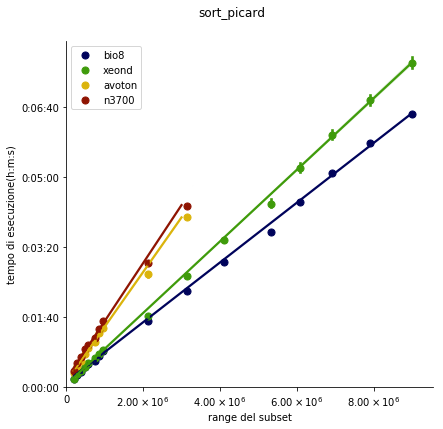
\includegraphics[scale=0.7]{sort_picard.png}
\captionof{figure}{Tempi per Sort Picard.}
\label{subfig:SP}
\end{figure}

\begin{table}[H]
    \centering
	\begin{tabular}{lrrrr}
	\toprule
	{} &         pendenza & intercetta &     min pendenza &     max pendenza \\
	\text{tipo di cpu} & $\frac{secondi}{\text{\text{\num{e6} letture}}}$ & $secondi$ & $\frac{secondi}{\text{\num{e6} letture}}$ & $\frac{secondi}{\text{\num{e6} letture}}$ \\			\midrule
	avoton   & 80 &        6.5 & 79 & 83 \\
	bio8     & 43 &        7.9 & 43 & 43 \\
	n3700    & 84 &         12 & 83 & 86 \\
	xeond    & 51 &        2.9 & 51 & 51 \\
	\bottomrule
	\end{tabular}
    \caption{Dettagli retta di fit per Sort Picard.}
    \label{tab:Sp}
\end{table}

La fase di riallineamento ha un comportamento differente dalle altre(realigner figura \ref{subfig:Rlg}), in quanto il tempo di avvio della regola, rappresentato dall'intercetta, costituisce una parte importante del tempo complessivo di esecuzione della regola stessa. 

Nei grafici sono distinguibili due gruppi di nodi significativamente diversi: avoton e n3700 contro xeond e bio8.
Questa distinzione è confermata dai valori delle pendenze riportate nelle tabelle \ref{tab:Bb}, \ref{tab:Mp}, \ref{tab:Md}, \ref{tab:Rlg} e \ref{tab:Sp}.
In particolare, il fatto che xeond e bio8 condividano lo stesso genere di architettura(tabella \ref{tab:cluster_generali}) indica come questa caratteristica possa influenzare l'esecuzione.

Infine, dai grafici si può notare che le regole di lunga durata sono il mapping e il realigner, mentre quella che impiega il minor tempo è il build bam.
Riguardo a mark duplicates e sort picard, si nota che queste regole condividono la stessa durata e la stessa crescita(tabelle \ref{tab:Md} e \ref{tab:Sp}).    


\subsection{Durata complessiva}
Un altro aspetto rilevato è stato il tempo complessivo richiesto per svolgere tutti i passaggi che esclusivamente dipendono dal numero di letture nel subset, escludendo tutti i passaggi non dipendenti (come l'indicizzazione del reference umano fatto da BWA).
Questi tempi sono rappresentativi del tempo richiesto per la pipeline per ciascun paziente. 

\begin{figure}[H]
\centering
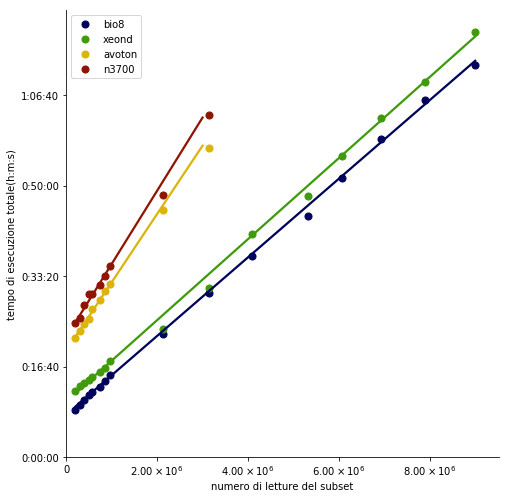
\includegraphics[scale=0.62]{Tempi_complessivi.png}	
\captionof{figure}{Tempi complessivi di esecuzione.}
\label{fig:Ttot}
\end{figure}

\begin{table}[H]
    \centering
	\begin{tabular}{lrrrr}
	\toprule
	{} &         pendenza &    intercetta &     min pendenza &     max pendenza \\
	\text{tipo di cpu} & $\frac{secondi}{\text{\num{e6} letture}}$ & $secondi$ & $\frac{secondi}{\text{\num{e6} letture}}$ & $\frac{secondi}{\text{\num{e6} letture}}$ \\
	\midrule
	avoton   &{760} & \num{1.2e+03} &{730} &{790} \\
	bio8     &{440} & \num{4.7e+02} &{440} &{440} \\
	n3700    & {800} & \num{1.3e+03} &{770} &{830} \\
	xeond    &{390} & \num{6.8e+02} &{390} & {400} \\
	\bottomrule
	\end{tabular}
    \caption{Pendenze per i tempi complessivi.}
    \label{tab:Ttot}
\end{table}

I grafici in figura \ref{fig:Ttot} e i valori in tabella \ref{tab:Ttot} confermano che i nodi sono separati in due coppie comparabili: avoton e n3700, xeond e bio8.


\subsection{Variabilità dei tempi di esecuzione}
Tutti i subset utilizzati nella sezione precedente condividono la stessa posizione iniziale di estrazione.
Per valutare la variabilità del tempo di esecuzione dalla posizione iniziale di estrazione, sono state ripetute le analisi con subset di stessa lunghezza ma con diversi punti di estrazione, tabella \ref{varT}.
Questi punti di estrazione sono stati scelti in modo da non aver sovrapposizione fra questi subset e il numero di letture stabilito è stato centomila.

\begin{table}[H]
\centering
\resizebox{1.0\textwidth}{!}{
\begin{tabular}{lrrrrr}
\toprule
regola & {build bam} & {mapping} & {mark duplicates} & {realigner} & {sort picard} \\
\text{tipo di cpu} &           &           &            &            &   \\
\midrule
avoton   &  $7.3\pm0.2$ &  $60\pm14$ & $16.4\pm0.3$ &  $1110\pm50$ &   $12.8\pm0.4$ \\
n3700    &  $8.00\pm0.18$ & $74\pm3$ & $18.4\pm0.8$ &  $1250\pm60$ &   $14.7\pm0.4$ \\
xeond    &  $3.27\pm0.07$ & $30\pm11$ &  $8.1\pm0.6$ &   $610\pm30$ &    $7.2\pm0.9$ \\
\bottomrule
\end{tabular}
}
\caption{Media e deviazione standard, espresse in secondi(s), dei tempi di esecuzione delle regole su diversi subset da centomila letture.}
\label{varT}
\end{table}

I dati associati a ciascuna regola indicano che i nodi tendenzialmente si stabilizzano su valori fissati.
Infatti, eccetto il mapping che mostra l'andamento meno stabile, i nodi impiegano la stessa quantità di tempo senza dipendere dal contenuto delle letture. 


\section{Memoria utilizzata}
La memoria occupata dai singoli processi è stata studiata analogamente al tempo, trascurando però lo studio di una memoria complessiva per tutti i passaggi. 
È stato analizzato in un primo momento l' occupazione della memoria per ognuna delle regole ed è poi stata stimata la variabilità di queste misure a partire da diverse posizioni iniziali.
La memoria intesa in questo capitolo si riferisce alla memoria "Resident Set Size" ricavata dal tool psutil e riportata da Snakemake, come già indicato nel paragrafo \ref{subsec:Mf}. 

\subsection{Consumo di memoria per le regole}
Le informazioni sui vari comportamenti sono tratte dai grafici nelle figure \ref{fig:BB_rss}, \ref{fig:Map_rss}, \ref{fig:MD_rss}, \ref{fig:Rlg_rss}, \ref{fig:SP_rss} e dalla tabella \ref{Tab:maxmem}.
\begin{figure}[H]
\begin{minipage}[b]{.5\textwidth}
\centering
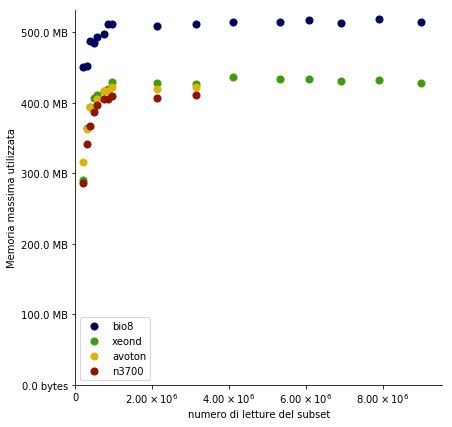
\includegraphics[width=0.9\textwidth]{Max_rss_build_bam.png}
\caption{Build BAM.}
\label{fig:BB_rss}
\end{minipage}
\hfill
\begin{minipage}[b]{.5\textwidth}
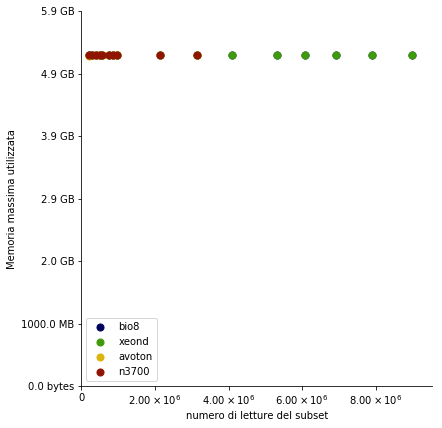
\includegraphics[width=0.9\textwidth]{Max_rss_mapping.png}
\caption{Mapping.}
\label{fig:Map_rss}	
\end{minipage}
\end{figure}

\begin{figure}[H]
\begin{minipage}[b]{.5\textwidth}
\centering
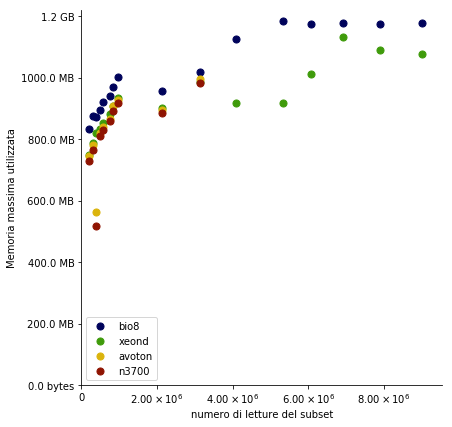
\includegraphics[width=0.9\textwidth]{Max_rss_mark_duplicates.png}
\caption{Mark Duplicates.}
\label{fig:MD_rss}
\end{minipage}
\hfill
\begin{minipage}[b]{.5\textwidth}
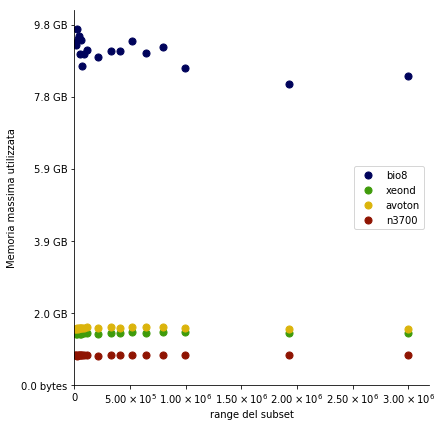
\includegraphics[width=0.9\textwidth]{Max_rss_realigner.png}
\caption{Realigner.}
\label{fig:Rlg_rss}	
\end{minipage}
\end{figure}

\begin{figure}[H]
\centering
\begin{minipage}[b]{.5\textwidth}
\centering
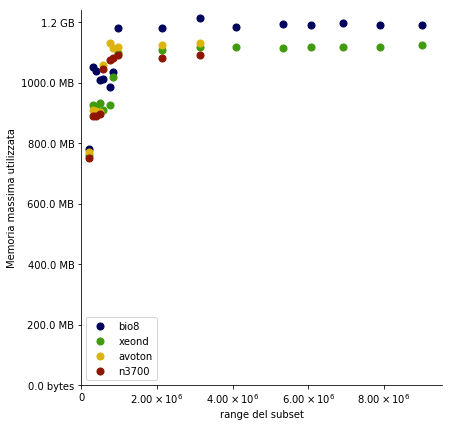
\includegraphics[width=0.9\textwidth]{Max_rss_sort_picard.png}
\caption{Sort Picard.}
\label{fig:SP_rss}
\end{minipage}
\end{figure}


\begin{table}[H]
\centering
\begin{tabular}{lrrrrr}
\toprule
regola &  \text{build bam} &  mapping &  \text{mark duplicates} &  realigner &  \text{sort picard} \\
\text{cpu type} &            &          &                  &            &              \\
\midrule
avoton   &        429 &     5305 &             1019 &       1626 &         1150 \\
bio8     &        527 &     5295 &             1042 &      10362 &         1232 \\
n3700    &        419 &     5306 &              988 &        859 &         1115 \\
xeond    &        435 &     5305 &             1004 &       1582 &         1138 \\
\bottomrule
\end{tabular}
\caption{Tabella dei massimi valori di memoria impiegati, espressi in MB.}
\label{Tab:maxmem}
\end{table}


Si può vedere che nelle regole di marcamento dei duplicati(figura \ref{fig:MD_rss}), di formazione del file BAM(figura \ref{fig:BB_rss}) e di riordimento per picard(figura \ref{fig:SP_rss}), la memoria satura una volta superato il milione di letture. 

Le altre regole che analizzano specificatamente i dati, la mappatura(figura \ref{fig:Map_rss}) e il riallineamento(figura \ref{fig:Rlg_rss}), hanno entrambe un'occupazione fissa della memoria.
Nel caso del mapping, infatti, tutte le macchine occupano la stessa quantità di memoria, indicando una saturazione generale, mentre nel riallineamento ciascuna cpu utilizza una quantità fissata di memoria che sembra essere una frazione della memoria totale disponibile. 

Per le regole che non dipendono dal paziente, riportate in figura \ref{fig:RSSind}, la richiesta di memoria non sembra invece dipendere significativamente dal nodo.

\begin{figure}[H]
\centering
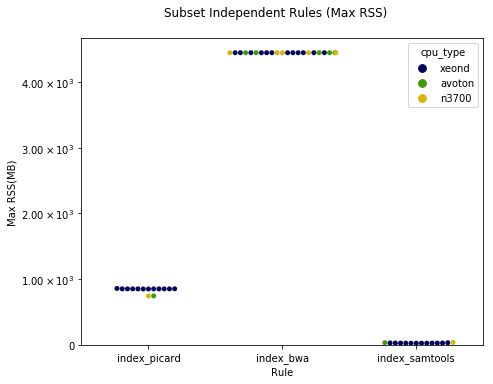
\includegraphics[scale=0.46]{Max_rss_ind.png}
\caption{Memoria impiegata dalle regole indipendenti dai subsets.}
\label{fig:RSSind}
\end{figure}

\subsection{Variabilità della memoria occupata}
Lo studio sulla memoria impiegata per intervalli diversi con ugual numero di sequenze è stato compiuto solo sui nodi dei cluster low power. 
La tabella \ref{fig:varM} riporta la media e la deviazione standard per ciascuna regola, su ogni nodo.
In particolare il numero di letture considerato è stato di centomila.

\begin{table}[H]
\centering
\resizebox{1.0\textwidth}{!}{
\begin{tabular}{lrrrrrrrrrr}
\toprule
regola & {build bam} & {mapping} & {mark duplicates} & {realigner} & {sort picard} \\
\text{tipo di cpu} &             &            &              &            &                 &           &            &            &             &           \\
\midrule
avoton   &  $240\pm8$ &  $5279.0\pm0.7$ & $702\pm7$ &  $1600\pm15$ & $585\pm3$ \\
n3700    &  $222\pm4$ &  $5280\pm6$ &  $686\pm7$ &   $830\pm11$ & $572\pm3$ \\
xeond    &  $230\pm12$ &  $5280\pm16$ &  $703\pm6$ &  $1430\pm30$ & $576\pm3$ \\
\bottomrule
\end{tabular}
}
\caption{Media e deviazione standard, espresse in MB, della memoria occupata dalle regole su diversi subset da centomila letture.}
\label{fig:varM}
\end{table}

I valori ottenuti evidenziano che la memoria è fortemente stabile in ogni regola, per ogni macchina.
Ciò conferma che le operazioni sfruttano la stessa quantità di memoria indipendentemente dal contenuto dei subset e, eccetto il caso del realigner, ne occupano pressochè lo stesso valore. 


%\section{Processi di I-O} 
%Gli ultimi risultati sono stati ottenuti dall'indagine sui processi di input e output coinvolti nel completamento di ogni lavoro.
%Questa sezione, sugli stessi modelli precedenti, è stata suddivisa in due parti che determinano come la lettura e la scrittura sono dipendenti dal set di dati e se il contenuto di tali dati incide sull'uso della macchina.
%
%\subsection{I-O e regole}
%Il primo esito riportato è per le regole indipendenti dai subset ed a parte l'indicizzazione per BWA l'impatto è praticamente nullo.
%\begin{figure}[H]
%\centering
%\subfloat[][\emph{Scrittura per regole indipendenti dai subset}]
%	{\label{subfig:Iind}
%	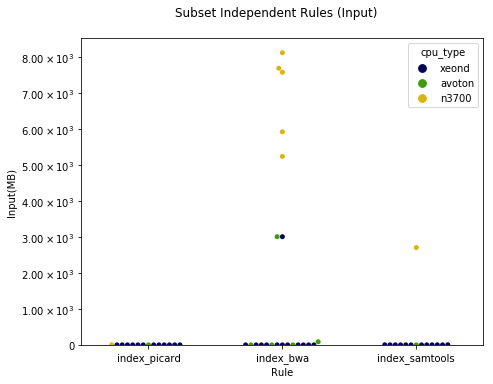
\includegraphics[width=.46\textwidth]{I_ind.png}
%	} \quad
%\subfloat[][\emph{Scrittura per regole indipendenti dai subset.}]
%	{\label{subfig:Oind}
%	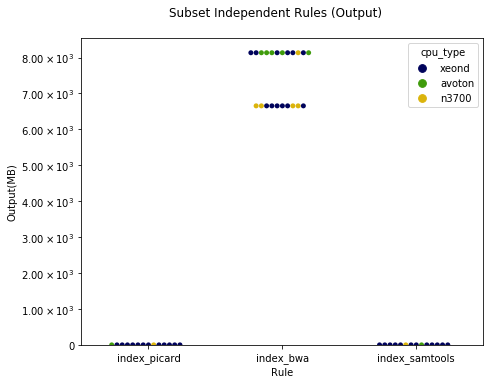
\includegraphics[width=.46\textwidth]{O_ind.png}
%	} \\
%\caption{}
%\label{fig:RSSrng}
%\end{figure}
%Diversamente dai tempi e dalla memoria, il lavoro di indicizzazione non è sempre costante sia per il caso di input che per quello dell'output.
%Riguardo all'input, le macchine più performanti (Xeon e Pentium N3700) nella maggior parte delle volte non eseguono alcuna lettura, mentre la rimanente varia in modo imprevedibile per valori elevati.
%Per l'output invece, l'andamento è costante per Pentium, al contrario di Xeon e Atom che similmente occupano due valori ben distinti. 
%
%
%Considerando le regole che invece dipendono dal subset, sono elecanti di seguito gli andamenti dei due processi per ognuna di esse.
%\begin{figure}[H]
%\centering
%\subfloat[][\emph{Lettura per la mappatura}]
%	{\label{subfig:IM}
%	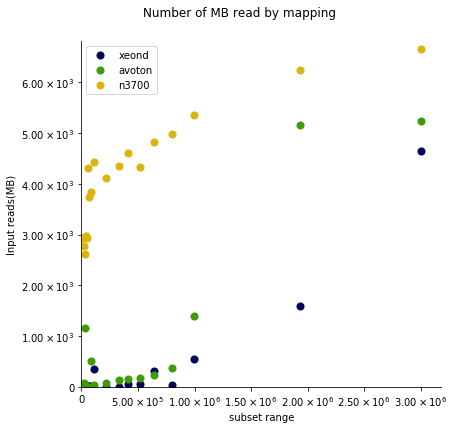
\includegraphics[width=.46\textwidth]{IO_Input_mapping.png}
%	} \quad
%\subfloat[][\emph{Scrittura per la mappatura}]
%	{\label{subfig:OM}
%	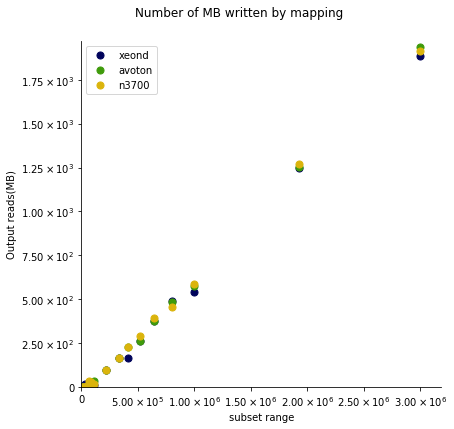
\includegraphics[width=.46\textwidth]{IO_Output_mapping.png}
%	} \\
%\caption{}
%\label{fig:IOm}
%\end{figure}
%
%La fase di lettura per la mappatura sembra crescere esponenzialmente per le due macchine migliori mentre per Pentium N3700 la crescita ha un andamento che tende a saturare in maniera logaritmica. 
%Gli elementi finali di Atom non seguono però un'esponenziale, suggerendo che avvenga una saturazione anche per le altre due macchine per grandezze dei subset superiori.
%
%La fase di scrittura, invece, mostra una andamento lineare praticamente omogeneo per tutte le macchine.  
%
%\begin{figure}[H]
%\centering
%\subfloat[][\emph{Lettura per il sorting di picard}]
%	{\label{subfig:ISp}
%	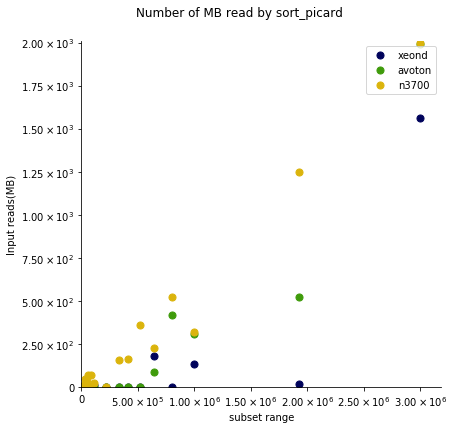
\includegraphics[width=.46\textwidth]{IO_Input_sort_picard.png}
%	} \quad
%\subfloat[][\emph{Scrittura per il sorting di picard}]
%	{\label{subfig:OSp}
%	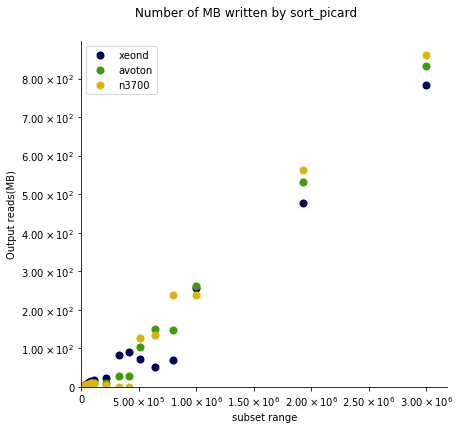
\includegraphics[width=.46\textwidth]{IO_Output_sort_picard.png}
%	} \\
%\caption{}
%\label{fig:IOSp}
%\end{figure}
%
%Per Picard il lavoro di riordinamento è ambiguo nella lettura perchè le macchine incrementano con traiettorie non ben definibili.
%Ad esempio, per Pentium la traiettoria potrebbe essere adattata ad una retta, ma esiste un certo sotto gruppo di dati che descrive una direzione nettamente diversa, così vanificando tale ipotesi.
%
%La scrittura invece inizia ad assumere contorni più chiari dopo una certa grandezza del subset, oltre il quale, tende a crescere linearmente. 
%Prima di raggiungere tale grandezza difatti ogni macchina, per numero di sequenze diversi, mostra un avvallamento non motivabile direttamente da questo tipo di studio statistico.  
%
%\begin{figure}[H]
%\centering
%\subfloat[][\emph{Lettura per la marcatura dei duplicati}]
%	{\label{subfig:IMd}
%	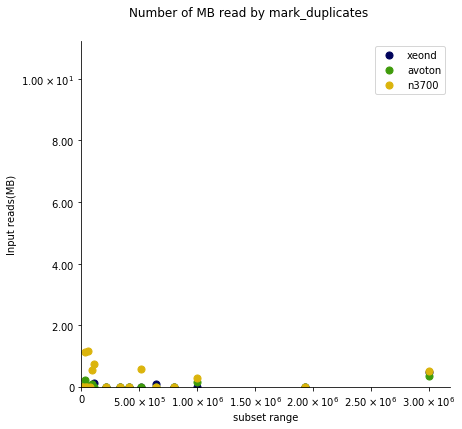
\includegraphics[width=.46\textwidth]{IO_Input_mark_duplicates.png}
%	} \quad
%\subfloat[][\emph{Scrittura per la marcatura dei duplicati}]
%	{\label{subfig:OMd}
%	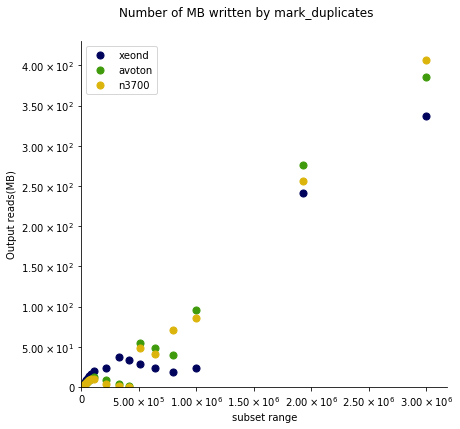
\includegraphics[width=.46\textwidth]{IO_Output_mark_duplicates.png}
%	} \\
%\caption{}
%\label{fig:IOMd}
%\end{figure}
%
%La descrizione della marcatura dei duplicati determina che la fase di lettura è coinvolta solo marginalmente, dato che esaurisce in generale meno di $2\,MB$, mentre quella di scrittura segue la stessa attitudine che il sorting per picard.
%Infatti ciò è evidente soprattutto in Xeon, per cui prima di avanzare con linearità è ben delineato un ventre di una curva.  
%
%\begin{figure}[H]
%\centering
%\subfloat[][\emph{Lettura per la formazione del BAM}]
%	{\label{subfig:IBB}
%	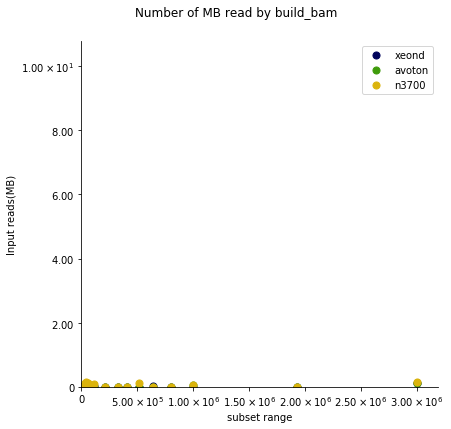
\includegraphics[width=.46\textwidth]{IO_Input_build_bam.png}
%	} \quad
%\subfloat[][\emph{Scrittura per la formazione del BAM}]
%	{\label{subfig:OBB}
%	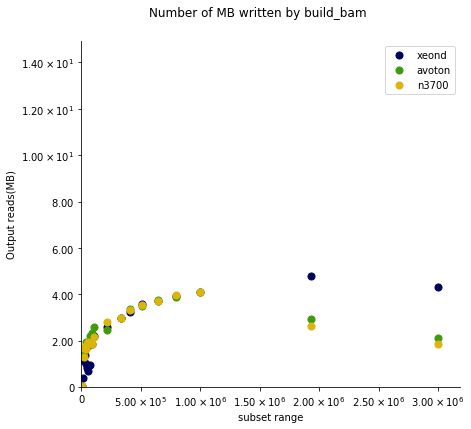
\includegraphics[width=.46\textwidth]{IO_Output_build_bam.png}
%	} \\
%\caption{}
%\label{fig:IOBB}
%\end{figure}
%
%Riguardo al passaggio per la costruzione dei file BAM, il numbero dei megabytes letti è trascurabile. 
%Al contrario, la scrittura segue una crescita logaritmica fino a circa 1 milione di subset, per poi cominciare a calare vistosamente.
%
%Le ragioni di questo calo non sono spiegabili, come nei casi precedenti, semplicemente osservando tale relazione dato che sarebbe più esauriente un approfindimento sia sulle prestazione dei macchinari che sul funzionamento dell'algoritmo di formazione del BAM. 
%
%\begin{figure}[H]
%\centering
%\subfloat[][\emph{Lettura per il riallineamento}]
%	{\label{subfig:IR}
%	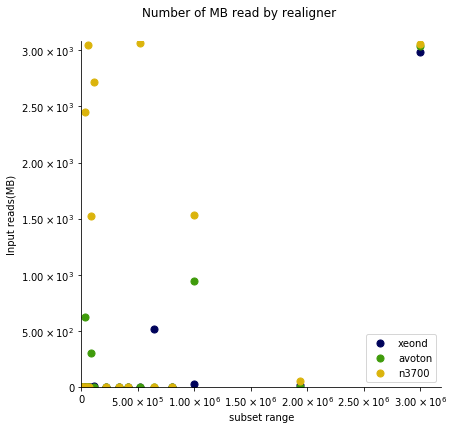
\includegraphics[width=.46\textwidth]{IO_Input_realigner.png}
%	} \quad
%\subfloat[][\emph{Scrittura per il riallineamento}]
%	{\label{subfig:OR}
%	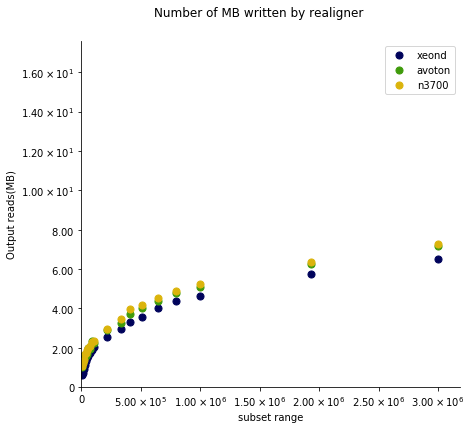
\includegraphics[width=.46\textwidth]{IO_Output_realigner.png}
%	} \\
%\caption{}
%\label{fig:IOR}
%\end{figure}
%
%In coda, il riallineamento mostra contemporaneamente il carattere meno comprensibile per la fase di lettura e quello più nitido per la fase di scrittura.
%I valori riportati nel grafico di input sono difficili da decifrare; non vi è un andamento univoco ne tra le cpu ne tra i dati associati ad ognuna di esse.
%Sono presenti un numero considerevole di processi che consumano una percentuale infinitesima in input che, però, sono alternati a salti elevati di letture, che tra loro non suggeriscono alcun andamento ben fissato.
%Evidentemente la natura del metodo di riallineamento influenza pesantemente questa fase di scansione dei bytes, riproducendo una lettura di essi fortemente discontinua.
%
%Nettamente diverso è il caso della scrittura, dove i dati tracciano una curva simile ad un logaritmo senza essere dotati di valori estranei ad essa.
%In più, i vari andamenti sono ordinati rispetto alla potenza computazionale delle macchine anche se, in questo frangente, con discrepanze molto sottili.
%
%\par Prima di passare al caso degli intervalli diversi con stesso intervallo, è utile sottolineare quali sono i lavori che generalemente consumano più bytes in fase di lettura e scrittura.
%In entrambi i casi è il mapping che vanta l'utilizzo maggiore e, all'opposto, è la formazione dei BAM che necessita del minor uso delle operazioni di input e output. 
%L'unico passaggio che presenta una netta inversione nell'uso di lettura e scrittura è, come si può controllare in figura \ref{fig:IOR}, il riallineamento, per cui sarà necessario uno studio specifico.
%
%\subsection{I-O per stessi range}
%L'ultima valutazione è stata eseguita, allo stesso modo che per i tempi e la memoria,  su intervalli diversi con lo stesso numero di letture.
%Sono stati scelti i grafici sottostanti per illustrare gli andamenti più interessanti ricavati durante le analisi.
%\begin{figure}[H]
%\centering
%\subfloat[][\emph{Input per realigner su range diecimila}]
%	{\label{subfig:IRdieci}
%	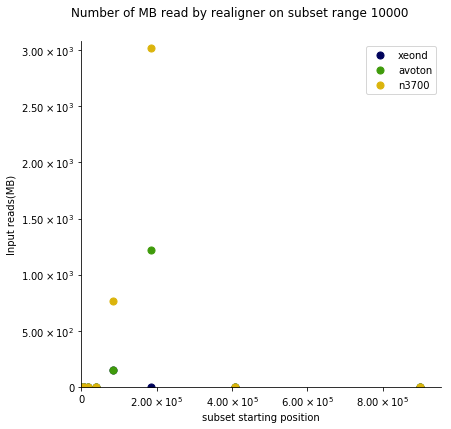
\includegraphics[width=.46\textwidth]{IO_I_realigner_dieci.png}
%	} \quad
%\subfloat[][\emph{Output per realigner su range diecimila}]
%	{\label{subfig:ORdieci}
%	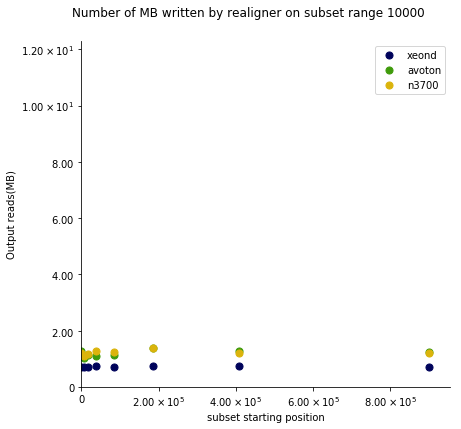
\includegraphics[width=.46\textwidth]{IO_O_realigner_dieci.png}
%	} \\
%\end{figure}
%\begin{figure}[H]
%\ContinuedFloat
%\centering
%\subfloat[][\emph{Input per mapping su range centomila}]
%	{\label{subfig:MIcento}
%	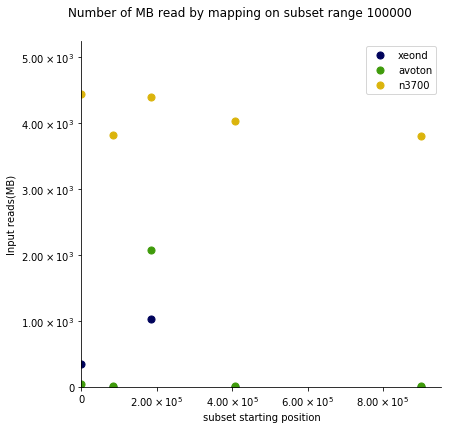
\includegraphics[width=.46\textwidth]{IO_I_map_cento.png}
%	} \quad
%\centering
%\subfloat[][\emph{Output per mapping su range centomila}]
%	{\label{subfig:MOcento}
%	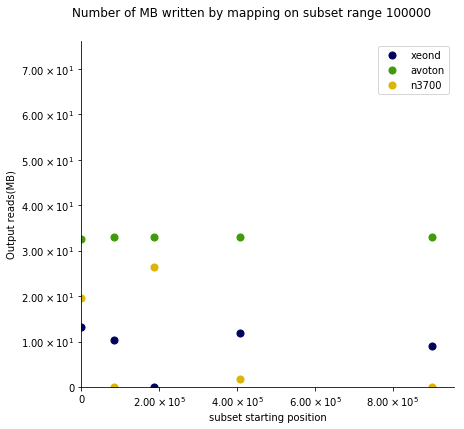
\includegraphics[width=.46\textwidth]{IO_O_map_cento.png}
%	} 
%\caption{}
%\label{fig:IOrng}
%\end{figure}
%
%I passaggi di scrittura mostrano un andamento più omogeneo per tipo di subset, pressochè costante nel caso della figura \ref{subfig:ORdieci} e per Atom(avoton) in \ref{subfig:ORdieci}.
%\'E interessante notare come le macchine computino con modalità diverse e che ciò causi la perdita dell'ordine delle cpu, dalla migliore alla peggiore, che caratterizzava le analisi per i tempi e la memoria.  
%
%Diverso è il caso della lettura che è rappresentato sia in \ref{subfig:IRdieci} che in \ref{subfig:MIcento}.  
%Le varie tracce non seguono andamenti ben definiti e sono spesso accompagnati da netti salti tra le misure di lettura, i quali inducono a pensare che sia il contenuto dei subset a determinare il tipo di lettura da svolgere. 
